\chapter{Tumbuhan yang Dijinakkan}\label{ch:g12:domesticated-plants}

Di samping tongkol jagung modern --- enam ratus butir dalam baris yang
rapi, terbungkus kelobot, melekat pada janggel yang tak akan
melepaskannya --- terbaring tongkol teosinte, rumput liar asalnya: dua
belas butir dalam satu baris, masing-masing bersarung cangkang sekeras
batu, rontok satu per satu ketika masak. Sembilan ribu tahun memilih,
oleh petani yang menyimpan benih tanaman yang mereka sukai, mengubah
yang satu menjadi yang lain. Hasilnya tak dapat bertahan satu musim
pun tanpa kita: tongkol jagung yang ditinggalkan di ladang membusuk di
tempatnya. Bab ini tentang apa yang terjadi pada tumbuhan ketika
manusia menjadi lingkungan yang menyeleksinya --- dan tentang cara
yang lebih baru untuk mengubah \omterm{def:g10:universal-dna:gene}{gen} tumbuhan dengan sengaja.

\section{Seleksi oleh manusia}

\begin{definition}[Domestikasi, seleksi buatan]\label{def:g12:domesticated-plants:domestication}
\emph{Domestikasi}\index{domestikasi} adalah perubahan sebuah \omterm{def:g10:biodiversity-scales:species}{spesies}
liar menjadi \omterm{def:g10:biodiversity-scales:species}{spesies} yang bergantung pada manusia dan melayaninya,
melalui \emph{seleksi buatan}\index{seleksi buatan}: pada setiap
generasi, orang menyimpan dan menyemai benih individu yang bersifat
seperti yang mereka inginkan, sehingga \omterm{def:g10:universal-dna:gene}{alel} di balik sifat itu naik
frekuensinya. Inilah seleksi \cref{ch:g12:selection-drift-speciation}
dengan mata manusia menggantikan lingkungan, dan ia bekerja dengan
hitungan yang sama --- lebih cepat, sebab pemilihannya sengaja dan
keras.
\end{definition}

\begin{proposition}[Apa yang diseleksi domestikasi]\label{prop:g12:domesticated-plants:traits}
Tanaman budidaya berbagi seperangkat sifat yang tak akan
dipertahankan tumbuhan liar mana pun, yaitu \emph{sindrom \omterm{def:g12:domesticated-plants:domestication}{domestikasi}}:
biji yang tetap melekat pada tanamannya alih-alih berhamburan (malai
yang tak rontok); biji dan buah yang lebih besar; biji yang berkecambah
seketika alih-alih menunggu bertahun-tahun di dalam tanah; hilangnya
racun dan pertahanan pahit; tanaman yang padat dengan sedikit cabang
dan satu tongkol besar alih-alih banyak tongkol kecil; serta pemasakan
yang serentak. Masing-masing berguna bagi pemanen dan merugikan bagi
tumbuhan yang berdiri sendiri --- tanaman budidaya adalah tumbuhan
yang diseleksi demi kemudahan kita dan melawan kemandiriannya.
\end{proposition}
\begin{proof}[Bukti percobaan]
Gandum liar merontokkan butirnya dari tangkai yang rapuh; gandum
budidaya yang paling awal, yang ditemukan di situs pertanian tertua,
punya tangkai liat yang menahan butirnya --- sabit sang pemanen, tanpa
sengaja, menyeleksi mutan yang butirnya tetap melekat pada tanaman
untuk dipungut dan disemai. Teosinte dan jagung hanya berbeda pada
sekitar lima \omterm{def:g10:universal-dna:gene}{gen} utama: satu mengubah tanaman bercabang banyak menjadi
satu batang, satu lagi membebaskan butirnya dari sarung batunya,
sisanya melipatgandakan barisnya. Menyilangkan keduanya memberi
keturunan yang subur, dan bentuk antaranya memang ada: \omterm{def:g10:biodiversity-scales:species}{spesies} yang
sama, yang dibentuk ulang.
\end{proof}

\begin{omfigure}
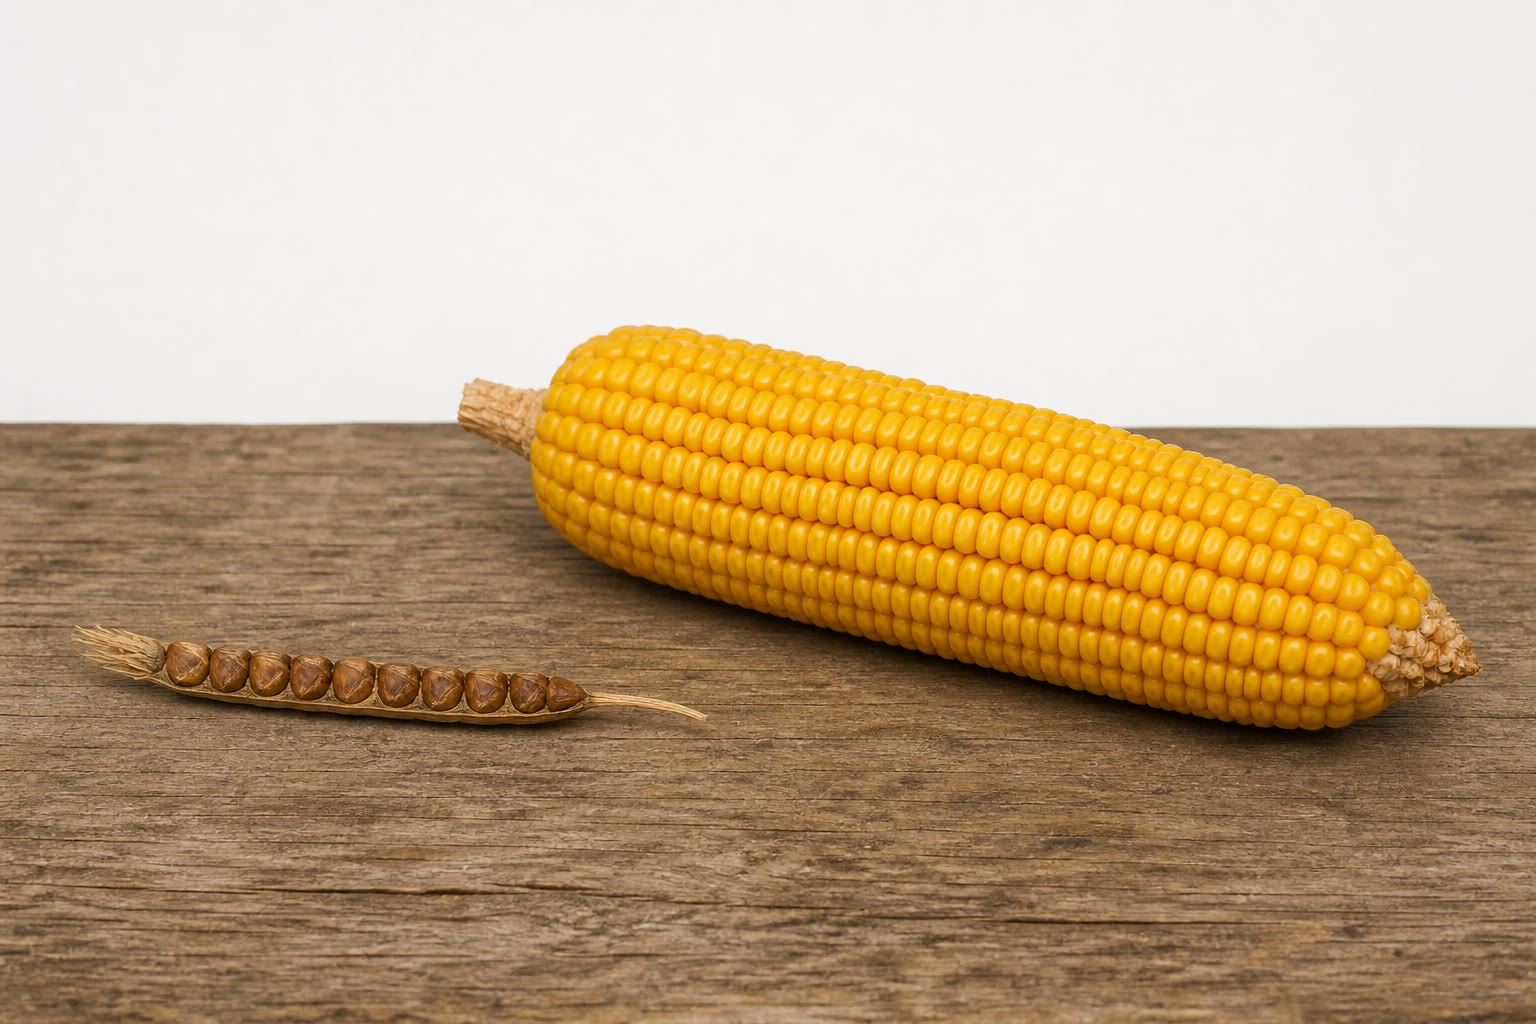
\includegraphics[width=0.62\linewidth]{images/book2/ai/g12-domestic-teosinte-maize.jpg}

{\small Teosinte dan jagung. Dua belas butir bersarung dalam satu
baris pada bulir yang rapuh, berhadapan dengan ratusan butir telanjang
yang melekat erat pada janggel: sembilan ribu tahun memilih, dan
segenggam \omterm{def:g10:universal-dna:gene}{gen}.}
\end{omfigure}

\begin{omfigure}
\begin{tikzpicture}[font=\small, >=Stealth,
  b/.style={draw, rounded corners, align=center, text width=2.2cm, minimum height=0.9cm}]
  \node[b, fill=omMeth!15, text width=2.8cm] (wild) at (0,0) {kubis liar\\ (satu spesies)};
  \node[b, fill=omDef!12] (kale) at (5,3.0) {kale:\\ daunnya};
  \node[b, fill=omDef!12] (cab) at (5,1.8) {kubis:\\ tunas ujungnya};
  \node[b, fill=omDef!12, text width=2.7cm] (spr) at (5,0.6) {kubis brussel:\\ tunas sampingnya};
  \node[b, fill=omDef!12] (kohl) at (5,-0.6) {kohlrabi:\\ batangnya};
  \node[b, fill=omDef!12] (broc) at (5,-1.8) {brokoli:\\ kuncup bunganya};
  \node[b, fill=omDef!12] (cauli) at (5,-3.0) {kembang kol:\\ tangkai bunganya};
  \foreach \t in {kale,cab,spr,kohl,broc,cauli} \draw[->] (wild.east) -- (\t.west);
  \node[anchor=west, align=left, text width=4.6cm] at (7.2,0) {Enam tanaman budidaya, satu spesies: pada tiap garis keturunan petani menyeleksi pembesaran organ yang berbeda. Keenamnya masih saling kawin.};
\end{tikzpicture}

{\small \omterm{def:g12:domesticated-plants:domestication}{Seleksi buatan} dari satu \omterm{def:g10:biodiversity-scales:species}{spesies} liar. Menyeleksi daun, tunas,
batang atau bunga pada garis keturunan yang berbeda menghasilkan
tanaman yang tampak seperti \omterm{def:g10:biodiversity-scales:species}{spesies} berbeda padahal bukan.}
\end{omfigure}

\begin{example}[Apa yang telah hilang dari tanaman budidaya]\label{ex:g12:domesticated-plants:lost}
Jagung tak dapat menghamburkan bijinya; gandum budidaya tak dapat
merontokkan butirnya; pisang dan anggur tanpa biji sama sekali tak
berbiji dan diperbanyak dengan setek, setiap tanamannya sebuah klon.
Kelangsungan hidup tanaman budidaya diserahkan kepada petani, dan
\emph{keragaman genetiknya} menyusut pada setiap tahap seleksi:
varietas modern nyaris seragam, dan satu wilayah utuh dapat menanam
satu varietas saja. Kerabat liarnya, yang masih beragam, adalah tempat
\omterm{def:g10:universal-dna:gene}{alel} yang mungkin diperlukan tanaman masa depan --- untuk penyakit
baru, untuk iklim yang lebih kering --- disimpan
(\cref{ch:g10:biodiversity-scales}).
\end{example}

\section{Pemuliaan dengan penyilangan}

\begin{proposition}[Varietas dan hibrida]\label{prop:g12:domesticated-plants:hybrids}
Pemulia membuat varietas baru dengan menyilangkan tanaman yang membawa
\omterm{def:g10:universal-dna:gene}{alel} berguna yang berbeda lalu menyeleksi, di antara keturunannya,
gabungan yang mereka inginkan, sepanjang beberapa generasi. Satu kasus
khusus menguasai jagung dan banyak sayuran: \emph{hibrida
F1}\index{hibrida F1}. Dua galur murni --- masing-masing dibuat seragam
dan homozigot oleh penyerbukan sendiri bergenerasi-generasi ---
disilangkan; keturunannya seluruhnya identik secara genetik,
heterozigot pada setiap \omterm{def:g10:universal-dna:gene}{gen} tempat kedua galur berbeda, dan jauh lebih
kuat serta produktif daripada kedua induknya. Bila disemai lagi, benih
hibrida itu memilah menjadi campuran tanaman yang kurang kuat: petani
membeli benih hibrida baru setiap tahun.
\end{proposition}
\admitted

\begin{omfigure}
\begin{tikzpicture}[font=\small, >=Stealth,
  b/.style={draw, rounded corners, align=center, text width=2.6cm, minimum height=1.0cm}]
  \node[b, fill=omDef!12] (a) at (0,1.2) {galur murni A\\ $AA\,bb$, seragam};
  \node[b, fill=omDef!12] (bb) at (0,-1.2) {galur murni B\\ $aa\,BB$, seragam};
  \node[b, fill=omMeth!20, text width=3.0cm] (f1) at (4.6,0) {hibrida F1\\ $Aa\,Bb$, semua identik,\\ kuat};
  \node[b, fill=omProp!15, text width=3.4cm] (f2) at (9.6,0) {F2 dari benih hibrida:\\ $AA$, $Aa$, $aa$ \dots bercampur,\\ hasil 15--20\% lebih rendah};
  \draw[->] (a) -- (f1); \draw[->] (bb) -- (f1);
  \draw[->] (f1) -- node[above] {disemai sendiri} (f2);
\end{tikzpicture}

{\small \omterm{prop:g12:domesticated-plants:hybrids}{Hibrida F1}. Dua galur homozigot memberi keturunan heterozigot
yang seragam dan sangat kuat; generasi berikutnya memilah dan
kehilangan kekuatan itu, sehingga benihnya harus dibeli lagi setiap
tahun --- dasar industri benih.}
\end{omfigure}

\begin{omfigure}
\begin{tikzpicture}
\begin{axis}[
  width=0.86\linewidth, height=5.6cm,
  axis x line=bottom, axis y line=left,
  xmin=1900, xmax=2025, ymin=0, ymax=9,
  xlabel={tahun}, ylabel={hasil gandum (t/ha)},
  xlabel style={font=\small, at={(axis description cs:0.5,-0.12)}, anchor=north},
  ylabel style={font=\small},
  tick label style={font=\small}, xtick={1900,1925,1950,1975,2000,2025}, ytick={0,2,4,6,8},
  clip=false,
]
\addplot[thick, omMeth, mark=*, mark size=1.5pt] coordinates
  {(1900,1.3) (1920,1.4) (1940,1.6) (1950,1.9) (1960,2.6) (1970,3.6) (1980,5.0) (1990,6.5) (2000,7.2) (2010,7.3) (2020,7.5)};
\draw[dashed, gray] (axis cs:1955,0) -- (axis cs:1955,8.5);
\node[font=\scriptsize, anchor=south, align=center] at (axis cs:1955,8.5) {varietas berjerami pendek,\\ pupuk, pestisida};
\end{axis}
\end{tikzpicture}

{\small Hasil gandum rata-rata di sebuah negara Eropa barat sepanjang
seabad (dibulatkan). Datar selama lima puluh tahun, lalu melipat empat
dalam empat puluh tahun berkat varietas baru yang dimuliakan agar
membawa malai berat pada batang pendek, bersama pupuk dan pengendalian
hama. Datarnya sejak 2000 adalah pokok pemuliaan masa kini.}
\end{omfigure}

\begin{example}[Mengapa hibrida itu kuat, dan mengapa kekuatannya tak bertahan]\label{ex:g12:domesticated-plants:vigour}
Setiap galur murni, yang homozigot di mana-mana, membawa beberapa \omterm{def:g10:universal-dna:gene}{alel}
\omterm{def:g11:genes-and-disease:genetic}{resesif} yang lemah dalam dosis ganda; menyilangkan dua galur
menyembunyikan \omterm{def:g10:universal-dna:gene}{alel} lemah tiap galur di balik \omterm{def:g10:universal-dna:gene}{alel} bekerja galur yang
lain, pada setiap \omterm{def:g10:universal-dna:gene}{gen} tempat keduanya berbeda. Karena itu F1 bersifat
heterozigot dan kuat. Pada generasi berikutnya, \omterm{def:g12:meiosis-genetic-shuffling:meiosis}{meiosis} dan pembuahan
membagikan \omterm{def:g10:universal-dna:gene}{alelnya} lagi
(\cref{ch:g12:meiosis-genetic-shuffling}): seperempat tanamannya
homozigot bagi \omterm{def:g10:universal-dna:gene}{alel} lemah pada tiap \omterm{def:g10:universal-dna:gene}{gen}, dan ladangnya menjadi
tambal sulam.
\end{example}

\section{Mengubah gen secara langsung}

\begin{proposition}[Tanaman transgenik dan tanaman suntingan]\label{prop:g12:domesticated-plants:transgenic}
Sejak 1980-an sebuah \omterm{def:g10:universal-dna:gene}{gen} dapat dimasukkan ke dalam tumbuhan tanpa
penyilangan: \emph{transgenesis}\index{transgenesis} (\cref{ch:g10:universal-dna}).
Sejenis bakteri tanah yang secara alami menyuntikkan sepotong \omterm{def:g10:universal-dna:information}{DNA-nya}
ke dalam \omterm{def:g10:cells-common-unit:cell}{sel} tumbuhan dipakai sebagai kendaraannya: \omterm{def:g10:universal-dna:gene}{gen} yang
diinginkan disisipkan ke dalam potongan itu, \omterm{def:g10:cells-common-unit:cell}{sel} tumbuhan diinfeksi,
dan tumbuhan utuh ditumbuhkan kembali dari \omterm{def:g10:cells-common-unit:cell}{sel} yang menerima \omterm{def:g10:universal-dna:gene}{gen}
tersebut. \omterm{def:g10:universal-dna:gene}{Gennya} boleh berasal dari \omterm{def:g10:biodiversity-scales:species}{spesies} mana pun. Belakangan ini,
\omterm{def:g10:universal-dna:gene}{gen} tumbuhan itu sendiri dapat diubah pada posisi yang dipilih ---
\emph{penyuntingan \omterm{def:g10:universal-dna:gene}{gen}} --- tanpa menambahkan \omterm{def:g10:universal-dna:information}{DNA} asing. Sifat yang
sudah ada: ketahanan terhadap serangga (sebuah \omterm{def:g10:universal-dna:gene}{gen} racun bakteri),
toleransi terhadap herbisida, ketahanan terhadap virus, prazat vitamin
pada padi, dan minyak dengan susunan yang diubah.
\end{proposition}
\admitted

\begin{omfigure}
\begin{tikzpicture}[font=\small, >=Stealth,
  b/.style={draw, rounded corners, align=center, text width=2.4cm, minimum height=1.0cm}]
  \node[b, fill=omThm!12] (gene) at (0,0) {gen yang diinginkan\\ (spesies mana pun)};
  \node[b, fill=omProp!15] (bact) at (3.3,0) {disisipkan ke dalam\\ DNA bakteri tanah\\ yang masuk ke tumbuhan};
  \node[b, fill=omDef!12] (cells) at (6.6,0) {sel tumbuhan diinfeksi;\\ sebagian menerima\\ gen itu};
  \node[b, fill=omMeth!15] (plant) at (9.9,0) {tumbuhan utuh ditumbuhkan\\ dari sel tersebut:\\ transgenik};
  \draw[->] (gene) -- (bact); \draw[->] (bact) -- (cells); \draw[->] (cells) -- (plant);
\end{tikzpicture}

{\small Membuat tumbuhan transgenik. Bakteri yang secara alami
menyisipkan \omterm{def:g10:universal-dna:information}{DNA} ke dalam \omterm{def:g10:cells-common-unit:cell}{sel} tumbuhan membawa masuk \omterm{def:g10:universal-dna:gene}{gen} yang dipilih;
tumbuhan ditumbuhkan kembali dari \omterm{def:g10:cells-common-unit:cell}{sel} yang menerimanya, dan
meneruskannya lewat bijinya.}
\end{omfigure}

\begin{example}[Sebuah gen racun di dalam jagung]\label{ex:g12:domesticated-plants:bt}
Sejenis bakteri tanah membuat \omterm{def:g11:gene-expression:protein}{protein} yang beracun bagi ulat dan tak
berbahaya bagi mamalia; \omterm{def:g10:universal-dna:gene}{gennya}, yang disisipkan ke dalam jagung,
membuat setiap \omterm{def:g10:cells-common-unit:cell}{sel} tanaman itu menghasilkan racun tersebut, dan ulat
penggerek yang melubangi batangnya mati pada gigitan pertamanya.
Penyemprotan insektisida berkurang; hasil panen naik di tempat
penggereknya parah. Dalam sepuluh tahun, penggerek yang \omterm{prop:g11:antibiotic-resistance:mechanisms}{tahan} terhadap
racun itu muncul di tempat tanaman ini ditanam tanpa jeda --- seleksi
\cref{ch:g11:antibiotic-resistance} di sebuah ladang --- dan petani
kini diwajibkan menyemai suaka jagung biasa di samping jagung
transgeniknya, agar penggerek yang peka tetap hidup untuk mengencerkan
penggerek yang \omterm{prop:g11:antibiotic-resistance:mechanisms}{tahan}.
\end{example}

\section{Pilihan}

\begin{proposition}[Apa yang dipertaruhkan]\label{prop:g12:domesticated-plants:stakes}
Setiap teknik dalam bab ini menimbulkan pertanyaan yang sama dalam
bentuk baru: menyempitnya keragaman (satu varietas di seluruh wilayah,
satu \omterm{def:g10:universal-dna:gene}{gen} di setiap tanaman), bergantungnya petani pada benih yang tak
dapat mereka simpan, terseleksinya hama dan gulma yang \omterm{prop:g11:antibiotic-resistance:mechanisms}{tahan} terhadap
pertahanan tanaman itu, menyebarnya \omterm{def:g10:universal-dna:gene}{gen} tanaman budidaya ke kerabat
liarnya lewat serbuk sari, serta keamanan dan kepemilikan apa yang
dimakan. Tak satu pun terjawab oleh biologi saja; biologi mengatakan
apa yang dikerjakan dan tidak dikerjakan setiap teknik, dan apa yang
diseleksinya.
\end{proposition}
\admitted

\begin{method}[Membaca riwayat sebuah tanaman budidaya]\label{met:g12:domesticated-plants:read}
\begin{enumerate}
  \item Kenali nenek moyang liarnya dan apa yang telah hilang dari
        tanaman budidaya itu dibandingkan dengannya (persebaran,
        dormansi, pertahanan, keragaman).
  \item Kenali bagaimana perubahannya dibuat: seleksi tak sadar lewat
        pemanenan, seleksi yang disengaja, penyilangan dan seleksi,
        hibridisasi, \omterm{prop:g10:universal-dna:universal}{transgenesis}, penyuntingan.
  \item Cacahlah \omterm{def:g10:universal-dna:gene}{gen} yang terlibat bila diketahui: beberapa \omterm{def:g10:universal-dna:gene}{gen} utama
        untuk sindrom \omterm{def:g12:domesticated-plants:domestication}{domestikasi}, banyak \omterm{def:g10:universal-dna:gene}{gen} kecil untuk hasil panen,
        satu \omterm{def:g10:universal-dna:gene}{gen} untuk sifat transgenik.
  \item Tanyakan pada apa tanaman itu kini bergantung (petani, benih
        yang dibeli, herbisida, suaka) dan apa yang bergantung padanya.
\end{enumerate}
\end{method}

\begin{remark}[Percobaan evolusi yang tertua]\label{rem:g12:domesticated-plants:oldest}
Darwin membuka bukunya tentang asal-usul \omterm{def:g10:biodiversity-scales:species}{spesies} dengan sebuah bab
tentang merpati dan kubis, sebab para pemulia sudah menunjukkan apa
yang dapat dikerjakan seleksi dalam beberapa abad; ia tinggal
menyingkirkan sang pemulia dan memanjangkan waktunya. Setiap tanaman
budidaya adalah peragaan tiga bab terakhir --- keragaman, seleksi, dan
perubahan frekuensi yang mengubah sebuah \omterm{def:g10:biodiversity-scales:species}{spesies} --- yang dijalankan
pada kecepatan manusia, dengan rekaman hasilnya di setiap ladang dan
setiap pasar.
\end{remark}

\section{Latihan}

\begin{exercise}[$\star$]\label{exo:g12:domesticated-plants:1}
Definisikan \omterm{def:g12:domesticated-plants:domestication}{domestikasi} dan \omterm{def:g12:domesticated-plants:domestication}{seleksi buatan}.
\end{exercise}

\begin{exercise}[$\star$]\label{exo:g12:domesticated-plants:2}
Sebutkan empat sifat sindrom \omterm{def:g12:domesticated-plants:domestication}{domestikasi} lalu katakan mengapa
masing-masing merugikan tumbuhan liar.
\end{exercise}

\begin{exercise}[$\star$]\label{exo:g12:domesticated-plants:3}
Apa itu \omterm{prop:g12:domesticated-plants:hybrids}{hibrida F1}, dan mengapa petani membeli benihnya setiap tahun?
\end{exercise}

\begin{exercise}[$\star$]\label{exo:g12:domesticated-plants:4}
Bagaimana sebuah \omterm{def:g10:universal-dna:gene}{gen} dimasukkan ke dalam tumbuhan tanpa penyilangan?
\end{exercise}

\begin{exercise}[$\star$]\label{exo:g12:domesticated-plants:5}
Dari gambar hasil panen, berapa kali lipat hasil gandum naik antara
1950 dan 2000?
\end{exercise}

\begin{exercise}[$\star\star$]\label{exo:g12:domesticated-plants:6}
Jelaskan bagaimana memanen dengan sabit, tanpa niat memuliakan sama
sekali, menyeleksi gandum bertangkai liat.
\end{exercise}

\begin{exercise}[$\star\star$]\label{exo:g12:domesticated-plants:7}
Kale, kubis dan brokoli saling kawin dengan bebas. Apakah ketiganya
satu \omterm{def:g10:biodiversity-scales:species}{spesies} atau tiga? Apa yang membuatnya tampak begitu berbeda?
\end{exercise}

\begin{exercise}[$\star\star$]\label{exo:g12:domesticated-plants:8}
Dua galur murni disilangkan. Pada sebuah \omterm{def:g10:universal-dna:gene}{gen} tempat galur A bergenotipe $AA$
dan galur B bergenotipe $aa$, sebutkan \omterm{def:g11:enzymes-and-phenotype:phenotype}{genotipe} F1 serta \omterm{def:g11:enzymes-and-phenotype:phenotype}{genotipe} dan
perbandingan F2. Mengapa F1 seragam dan F2 tidak?
\end{exercise}

\begin{exercise}[$\star\star$]\label{exo:g12:domesticated-plants:9}
Mengapa penggerek yang \omterm{prop:g11:antibiotic-resistance:mechanisms}{tahan} muncul di ladang jagung penghasil racun,
dan bagaimana suaka jagung biasa memperlambatnya?
\end{exercise}

\begin{exercise}[$\star\star$]\label{exo:g12:domesticated-plants:10}
Teosinte dan jagung berbeda pada sekitar lima \omterm{def:g10:universal-dna:gene}{gen} utama. Jelaskan
bagaimana \omterm{def:g10:universal-dna:gene}{gen} sesedikit itu dapat mengubah tanaman sebesar itu, dengan
memakai \cref{ch:g12:diversification-of-life}.
\end{exercise}

\begin{exercise}[$\star\star$]\label{exo:g12:domesticated-plants:11}
Mengapa kerabat liar tanaman budidaya dilestarikan di bank benih,
padahal hasil panennya hampir nihil?
\end{exercise}

\begin{exercise}[$\star\star\star$]\label{exo:g12:domesticated-plants:12}
Kanola yang toleran herbisida ditanam di sebelah sesawi liar yang
dapat disilanginya. Ramalkan apa yang mungkin terjadi selama beberapa
tahun, dan sebutkan proses bab terdahulu yang terlibat.
\end{exercise}

\begin{exercise}[$\star\star\star$]\label{exo:g12:domesticated-plants:13}
Kurva hasil panennya datar sejak 2000. Usulkan dua alasan biologis dan
satu alasan nonbiologis, lalu katakan apa yang mungkin dicoba seorang
pemulia.
\end{exercise}

\begin{exercise}[$\star\star\star$]\label{exo:g12:domesticated-plants:14}
Bandingkan, pada tiga butir, varietas yang diperoleh dengan
penyilangan dan seleksi terhadap varietas yang diperoleh dengan
\omterm{prop:g10:universal-dna:universal}{transgenesis}: asal \omterm{def:g10:universal-dna:gene}{alel} barunya, jumlah \omterm{def:g10:universal-dna:gene}{gen} yang diubah, dan waktu
yang diperlukan.
\end{exercise}

\begin{exercise}[$\star\star\star$]\label{exo:g12:domesticated-plants:15}
``\omterm{def:g12:domesticated-plants:domestication}{Domestikasi} adalah kebalikan \omterm{def:g12:selection-drift-speciation:selection}{seleksi alam}.'' Bahaslah dalam satu
paragraf dengan hitungan \omterm{def:g12:selection-drift-speciation:population}{frekuensi alel}, pelaku seleksinya, dan nasib
tumbuhan yang diseleksi itu.
\end{exercise}

\section{Soal: Sembilan Ribu Tahun, Lima Gen}

\begin{problem}[{Soal akhir pekan --- jagung yang dibuat dari teosinte:
tongkolnya dibandingkan, seleksinya dihitung, hasil sebuah hibrida
diikuti sampai F2, dan sebuah gen racun dikelola melawan ketahanan}]
\label{pb:g12:domesticated-plants:1}
Sebuah bulir teosinte membawa 12 butir seberat \qty{0.08}{g},
bersarung cangkang keras, pada poros yang rapuh; sebuah tongkol jagung
membawa 600 butir seberat \qty{0.3}{g}, telanjang, pada janggel yang
kaku. Jagung didomestikasi sekitar 9000 tahun lalu; satu generasi satu
tahun.

\medskip
\noindent\textbf{Bagian I --- Tongkolnya.}
\begin{enumerate}
  \item Hitunglah massa butir per tongkol pada teosinte dan pada
        jagung, serta kelipatan di antara keduanya.
  \item Sebutkan sifat tongkol jagung yang termasuk sindrom
        \omterm{def:g12:domesticated-plants:domestication}{domestikasi}, dan untuk masing-masing katakan mengapa sifat itu
        akan merugikan tumbuhan liar.
  \item Butir bersarung dikendalikan oleh satu \omterm{def:g10:universal-dna:gene}{gen}, dengan \omterm{def:g10:universal-dna:gene}{alel}
        telanjang bersifat \omterm{def:g11:genes-and-disease:genetic}{resesif}. Jelaskan mengapa petani pertama
        hanya dapat menemukan tanaman berbutir telanjang sebagai
        individu yang langka di ladangnya.
  \item Andaikan \omterm{def:g10:universal-dna:gene}{alel} telanjang berfrekuensi 0.01 pada \omterm{def:g12:selection-drift-speciation:population}{populasi}
        liarnya. Berapa bagian tanaman yang menampakkan butir
        telanjang?
  \item Seorang petani hanya menyemai benih dari tanaman berbutir
        telanjang. Berapa \omterm{def:g12:selection-drift-speciation:population}{frekuensi alel} telanjang pada panennya
        berikutnya?
\end{enumerate}

\medskip
\noindent\textbf{Bagian II --- Sembilan ribu generasi.}
\begin{enumerate}[resume]
  \item Jumlah butir per tongkol naik dari 12 menjadi 600 sepanjang
        9000 generasi. Hitunglah kelipatan kenaikan rata-rata tiap
        generasi. Mengapa perubahan sekecil itu tiap generasi sudah
        cukup?
  \item Jumlah baris butir dikendalikan oleh banyak \omterm{def:g10:universal-dna:gene}{gen} berefek kecil.
        Jelaskan mengapa sifat semacam itu menanggapi seleksi secara
        berangsur dan lama, sedangkan sifat butir bersarung berubah
        dalam satu langkah.
  \item Jagung masih dapat disilangkan dengan teosinte dan memberi
        keturunan yang subur. Apakah keduanya satu \omterm{def:g10:biodiversity-scales:species}{spesies}? Apa yang
        telah diubah dan tidak diubah oleh \omterm{def:g12:domesticated-plants:domestication}{domestikasi}?
  \item Sebuah varietas modern seragam secara genetik. Nyatakan risiko
        yang mengikutinya, dan sumber daya yang menjawabnya.
  \item Jagung tak dapat menyebarkan bijinya. Apa artinya hal ini bagi
        hubungan antara tanaman itu dan petaninya, dalam istilah
        seleksi?
\end{enumerate}

\medskip
\noindent\textbf{Bagian III --- Hibridanya.}
Galur murni A berhasil \qty{5}{t/ha}, galur B \qty{5.5}{t/ha}, \omterm{prop:g12:domesticated-plants:hybrids}{hibrida
F1} keduanya \qty{10}{t/ha}; F2 yang ditanam dari benih hibrida itu
berhasil \qty{8.2}{t/ha}. Benih hibrida berharga setara \qty{0.4}{t/ha}
jagung.
\begin{enumerate}[resume]
  \item Berapa persen F1 melampaui induknya yang lebih baik? Berapa
        persen F2 jatuh di bawah F1?
  \item Jelaskan kekuatan F1 dan kemerosotan F2 dengan \omterm{def:g11:enzymes-and-phenotype:phenotype}{genotipe} pada
        \cref{ex:g12:domesticated-plants:vigour}.
  \item Seorang petani ragu antara membeli benih hibrida setiap tahun
        dan menyimpan benih dari F1. Bandingkan panen bersihnya, lalu
        katakan mengapa usaha perusahaan benih itu ada.
  \item Mengapa galur murninya tidak dijual saja kepada petani agar
        mereka membuat hibridanya sendiri?
  \item Apa yang telah dilakukan sistem hibrida itu terhadap keragaman
        genetik ladang, dan terhadap kemandirian petaninya?
\end{enumerate}

\medskip
\noindent\textbf{Bagian IV --- \omterm{def:g10:universal-dna:gene}{Gen} racunnya.}
Sebuah \omterm{def:g12:selection-drift-speciation:population}{populasi} penggerek punya \omterm{def:g10:universal-dna:gene}{alel} ketahanan berfrekuensi 0.001,
bersifat \omterm{def:g11:genes-and-disease:genetic}{resesif}; hanya penggerek $rr$ yang selamat pada jagung beracun.
\begin{enumerate}[resume]
  \item Berapa bagian penggerek yang selamat di ladang jagung beracun
        pada tahun pertama? Hitunglah frekuensi $r$ di antara para
        penyintasnya.
  \item Jelaskan mengapa, tanpa suaka, ketahanan itu menyebar dalam
        beberapa tahun, dengan memakai kasus \omterm{def:g11:antibiotic-resistance:antibiotic}{antibiotik} sebagai model.
  \item Sebuah suaka jagung biasa menjaga \omterm{def:g12:selection-drift-speciation:population}{populasi} besar penggerek
        peka tetap hidup di sebelah ladang beracunnya. Jelaskan
        bagaimana hal itu menjaga \omterm{def:g10:universal-dna:gene}{alel} ketahanan tetap jarang, dengan
        memakai \omterm{def:g11:enzymes-and-phenotype:phenotype}{genotipe} keturunan seekor penyintas yang \omterm{prop:g11:antibiotic-resistance:mechanisms}{tahan} dan
        seekor penggerek dari suaka.
  \item Bandingkan suaka itu dengan ``kur penuh'' \omterm{def:g11:antibiotic-resistance:antibiotic}{antibiotik}: apa yang
        sama, apa yang berbeda?
  \item Nyatakan hasilnya: kelipatan yang dipakai \omterm{def:g12:domesticated-plants:domestication}{domestikasi} untuk
        melipatgandakan butir sebuah tongkol, jumlah \omterm{def:g10:universal-dna:gene}{gen} utama yang
        diperlukannya, dan satu ketergantungan yang diciptakannya.
\end{enumerate}
\end{problem}
